\subsection{The Standard Model}
The Standard Model of particle physics represents the most complete description of fundemental interactions to date, surviving over 70+ years of theoratical and experimental scrutiny.
The Standard Model, shown in Figure~\ref{fig:standard_model_particles}, combines Quantum Field Theories of the ElectroWeak forces (Electrodynamics) and the Strong interaction (Chromodynamics) into a unified framework.
Each interaction has its own force carrier, with the strong, electromagnetic, and weak forces being mediated by the gluon, photon, and W$^{\pm}$+Z bosons respectivly.


\begin{figure}
    \centering
    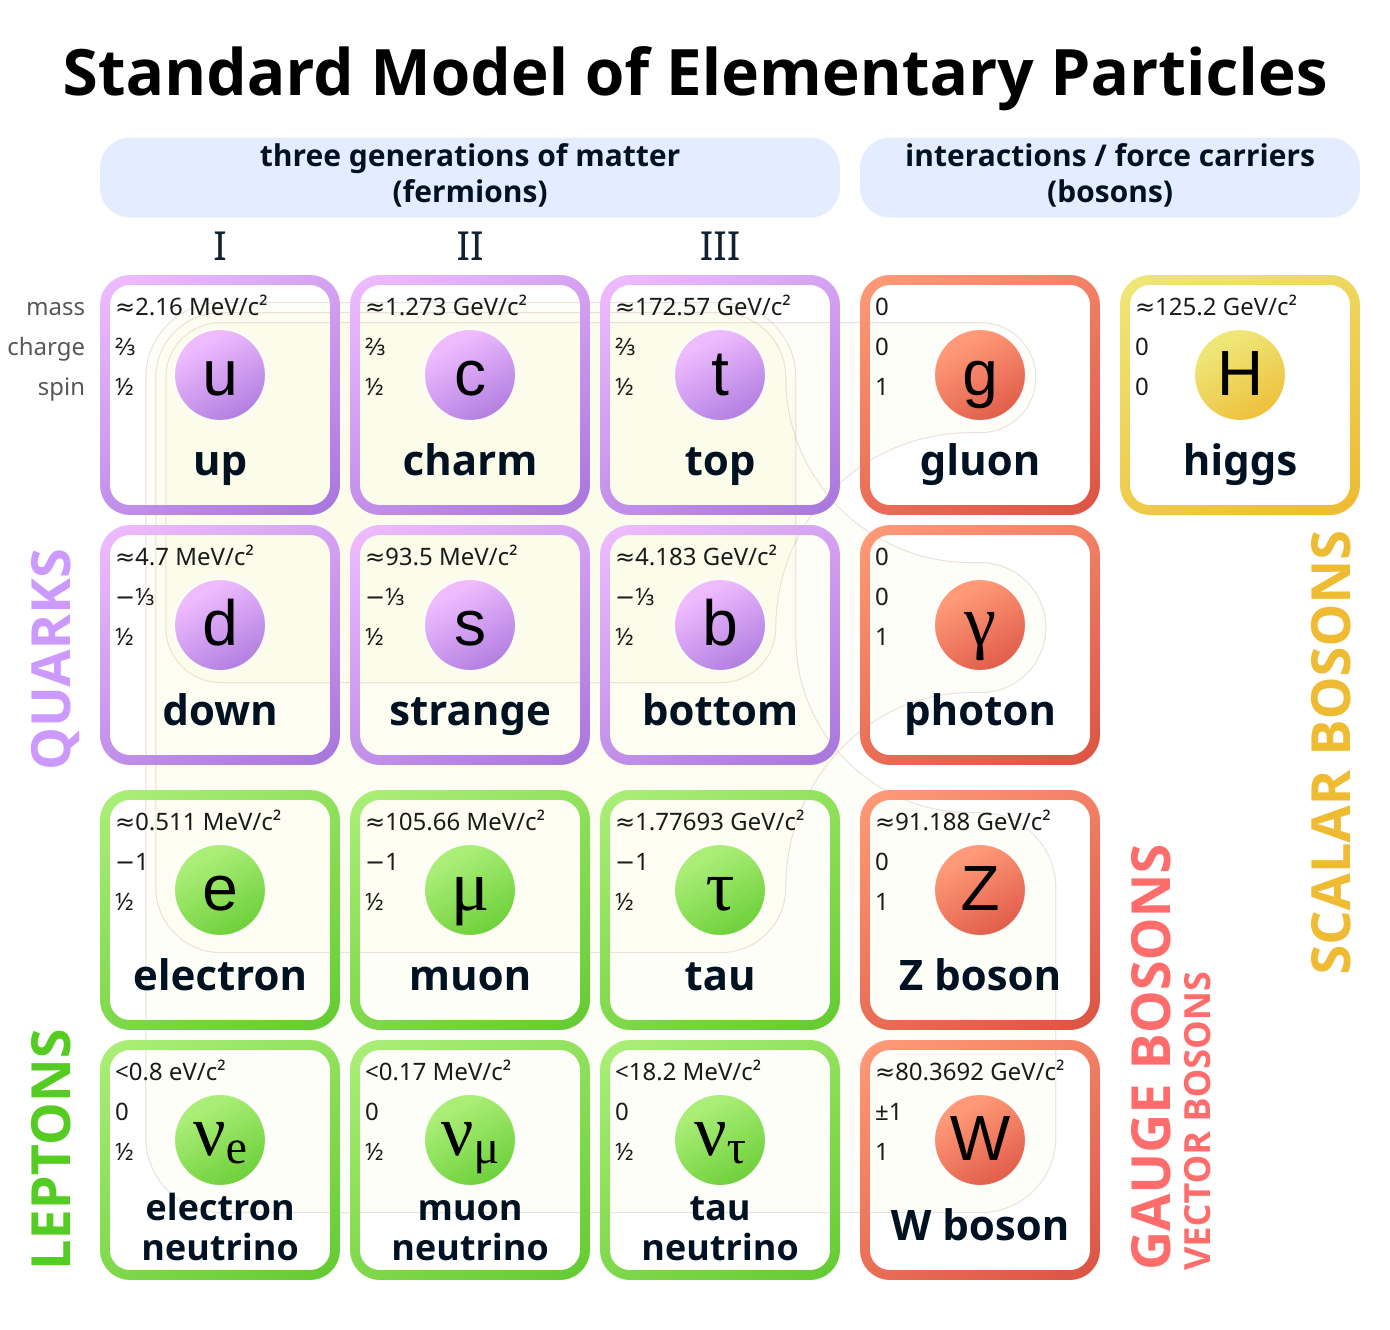
\includegraphics[
        width=0.85\textwidth,
        alt={Diagram of the Standard Model showing three generations of quarks
        and leptons, along with gauge bosons and the Higgs boson.}
    ]{chapters/introduction/figures/the_standard_model/standard_model_of_elementary_particles.pdf}
    \caption{The elementary particles and force carriers of the Standard Model.
    Adapted from Ref.~\cite{WikimediaCommonsStandardModel}.}
    \label{fig:standard_model_particles}
\end{figure}
